\documentclass[conference]{IEEEtran}
\usepackage[T1]{fontenc}
\usepackage{amsmath}
\usepackage{amssymb}
\usepackage{graphicx}
\usepackage{xcolor}
\usepackage{cite}
\usepackage{url}
\usepackage{algorithm}
\usepackage{algorithmic}
\usepackage{booktabs}
\usepackage{multirow}
\usepackage{hyperref}
\graphicspath{{figures/}}

\begin{document}

\title{Persistent Fact-Slot Memory for LLM Agents: A Pilot Study of Cost, Retention, and Scaling Limits}

\author{\IEEEauthorblockN{Ishan Gautam}
\IEEEauthorblockA{
\textit{Pulchowk Campus} \\
\textit{Institute of Engineering, Tribhuvan University} \\
Lalitpur, Nepal \\
080bct034.ishan@pcampus.edu.np
}
\and
\IEEEauthorblockN{Kushal K.C.}
\IEEEauthorblockA{
\textit{Pulchowk Campus} \\
\textit{Institute of Engineering, Tribhuvan University} \\
Lalitpur, Nepal \\
080bct041.kushal@pcampus.edu.np
}
}

\maketitle

\begin{abstract}
Large language model (LLM) agents incur token costs that grow super-linearly with conversation length because each step may re-send an expanding history. Persistent external memory is often proposed as a remedy, but its retention/cost trade-off is easy to overstate. This paper studies \emph{persistent fact-slot memory}, a hierarchical architecture in which a small model extracts durable facts into latest-value subject--predicate slots and a larger model answers from that slot table plus a recent-message window. We formalize the cost model, specify the Fact-Slot representation, release a reproducible evaluation harness, and report live Groq evaluations on 30 synthetic conversations spanning 14--200 messages. Fact-Slot Memory retains 84.0\% of planted facts, reduces real input tokens by 58.8\%, and costs 63.3\% of full context, improving over append-only notes (54.6\% retention, 45.6\% token reduction, 77.7\% cost). Per-length-class analysis reveals the asymptotic advantage: at 200 messages, Fact-Slot Memory costs only 26.8\% of full-context cost while retaining 86.7\% of facts. Running-summary baselines achieve perfect retention at all lengths but cost more (104.0\% overall). These results demonstrate that latest-value structured memory can improve the cost--retention frontier over append-only representations and that the advantage grows with conversation length.
\end{abstract}

\begin{IEEEkeywords}
large language model agents, fact-slot memory, LLM cost optimization, conversation summarization, persistent memory, model cascading, token-efficient prompting, hierarchical memory, long-context management, prompt compression, retrieval-augmented memory, agentic systems
\end{IEEEkeywords}

\section{Introduction}

Autonomous AI agents have revolutionized tasks ranging from market intelligence to sales outreach, yet their economic viability remains challenged by escalating token costs. While a single-sentence interaction may span on the order of 1,000 tokens in practice, autonomous agents routinely perform multi-step reasoning, tool calls, and context re-stacking that can consume tens of thousands of tokens per task \cite{zhou2024agents, shinn2023reflexion, park2023generative}.

The problem intensifies as conversations lengthen. When agents include more history in each step, cumulative token costs over a multi-turn task can grow quadratically rather than linearly. Poorly architected agents can consume resources at unsustainable rates once retry rates, parallel instances, and tool overhead are accounted for \cite{shinn2023reflexion}. Simply enlarging the context window is not a free remedy: long-context models exhibit a ``lost in the middle'' effect, where content placed away from the prompt's ends is under-utilized \cite{nfliu2023lost}, and self-attention makes additional tokens more expensive in compute \cite{packer2023memgpt}.

Current mitigation strategies include:
\begin{enumerate}
    \item \textbf{Semantic Caching}: Reuse outputs for semantically similar inputs \cite{bang2023gptcache}.
    \item \textbf{History Summarization}: Compress past conversations into running summaries to bound context length \cite{sung2024wmt}.
    \item \textbf{Model Cascading}: Use small models for easy sub-tasks and escalate to expensive models only when required \cite{chen2023frugalgpt}.
    \item \textbf{Prompt Compression}: Drop low-information tokens before inference using a small scoring model \cite{jiang2023llmlingua}.
    \item \textbf{Hierarchical / Virtual Memory}: Page information in and out of the context window from external storage \cite{packer2023memgpt}.
\end{enumerate}

However, existing approaches face limitations. Naive truncation discards critical information indiscriminately. Aggressive summarization may drop important details \cite{sung2024wmt}. Semantic caching only helps when queries repeat. Prompt compression operates at the token level and does not produce a durable, queryable record of the conversation. Crucially, most summarization implementations use the \emph{same} expensive model for both compression and synthesis, leaving the largest cost-saving lever -- a cheap extractor -- untouched. Prior work on agent memory highlights the need for structured, persistent approaches beyond simple summarization \cite{park2023generative, zhong2024memorybank, zhang2024memorysurvey}.

\textbf{Our Contribution}: This paper proposes and stress-tests a \textit{hierarchical Fact-Slot memory architecture} that combines model cascading with structured history summarization. A small model extracts durable facts from conversation segments, upserts them into a persistent latest-value slot table, and subsequent prompts reference this compact table alongside only recent messages. Concretely, this paper makes the following contributions:
\begin{enumerate}
    \item A token-cost model that makes explicit why full-context agents scale quadratically over a multi-turn task, and a retention requirement that formalizes the information an agent must preserve (Section~\ref{sec:problem}).
    \item A persistent memory architecture that applies the model-cascading insight to the \emph{memory} step -- a cheap extractor writes latest-value fact slots, an expensive model only synthesizes -- together with concrete schemas and extraction prompts (Section~\ref{sec:method}).
    \item An evaluation protocol -- metrics, baselines, and a synthetic conversation suite -- for measuring token reduction, cost, retention accuracy, update retention, and answer quality (Section~\ref{sec:experiments}).
    \item An open-source reference implementation released as a research repository (Section~\ref{sec:implementation}).
\end{enumerate}
The append-only notes design is retained as a comparison baseline because it targets raw token reduction while preserving retention accuracy; our sweep evaluation (Section~\ref{sec:results}) shows append-only notes degrade at longer horizons due to unbounded growth and lack of contradiction resolution. The Fact-Slot design improves the measured frontier across all length classes and, unlike running-summary, its cost advantage grows with conversation length. We release all artifacts to support reproducibility and extension.

\section{Related Work}

Memory optimization for LLM agents has emerged as a critical research area; a recent survey systematizes the design space of agent memory across short-term context, long-term storage, and the read/write mechanisms that connect them \cite{zhang2024memorysurvey}. We position our contribution within three adjacent lines of work: prompt compression, model cascading, and persistent agent memory.

\textbf{Prompt and context compression.} LLMLingua uses a small language model to score and remove low-information tokens from a prompt in a coarse-to-fine manner, achieving up to $20\times$ compression with limited performance loss \cite{jiang2023llmlingua}. This validates the central premise that a cheap model can identify what matters, but compression is ephemeral -- it rewrites a single prompt and leaves no reusable record of the conversation. The motivation for compression is reinforced by evidence that models do not use long contexts uniformly: relevant content placed in the middle of a long prompt is systematically underused \cite{nfliu2023lost}.

\textbf{Model cascading.} FrugalGPT demonstrates that routing queries through a cascade of progressively more expensive models can match GPT-4 quality at up to 98 percent lower cost \cite{chen2023frugalgpt}. Cascading is highly effective for answering, but prior cascades target the \emph{response} step rather than the \emph{memory} step; they do not use the cheap model to maintain long-term state. Our work applies the cascade insight specifically to extraction-and-storage.

\textbf{Persistent agent memory.} Park et al. introduce Generative Agents, whose memory stream and retrieval support coherent long-horizon behavior, but their focus is believable simulation rather than cost \cite{park2023generative}. Zhong et al. propose MemoryBank, a dynamic memory-updating mechanism for LLMs that shares our persistence goal but uses a single model and does not exploit cascading \cite{zhong2024memorybank}. MemGPT frames the context window as virtual memory, paging information between an in-context tier and external storage via function calls \cite{packer2023memgpt}; our fact-slot table is a deliberately simpler realization of the same external-memory idea, with the added emphasis that writes are performed by a cheaper model. Recent conversation-summarization systems combine recent dialogue with a running summary of earlier turns \cite{sung2024wmt}, but typically employ a single model without separating cheap extraction from expensive synthesis. Our work bridges these gaps by combining structured extraction by a small model, persistent latest-value storage, and selective context retrieval with explicit overwrites for updated facts.

\section{Problem Formulation}
\label{sec:problem}

\subsection{Token Cost Growth Model}

Let $C(n)$ denote the token cost for a conversation with $n$ messages. In traditional approaches where full history is retained:

\begin{equation}
C(n) = \alpha_{\text{large}} \cdot \sum_{i=1}^{n} \text{tokens}(m_i) + \beta_{\text{large}} \cdot \text{tokens}(m_{\text{out}})
\end{equation}

where $\alpha_{\text{large}}$ represents the input cost per token for the large model (typically \$0.003 to \$0.005 per 1,000 tokens), $\beta_{\text{large}}$ represents the output cost per token, $m_i$ denotes the $i$-th message, and $m_{\text{out}}$ represents the generated response.

Since $\sum_{i=1}^{n} \text{tokens}(m_i)$ grows linearly with $n$, and each API call includes this cumulative context, the total cost for $k$ conversation turns grows approximately as:

\begin{equation}
\text{Total Cost}_{\text{full}}(k) \approx \sum_{j=1}^{k} C(j) \propto k^2
\end{equation}

For example, if each turn adds roughly $b$ input tokens and output length is treated as a lower-order term, then $C(j) \approx \alpha_{\text{large}} b j$ and
\begin{equation}
\sum_{j=1}^{k} C(j) \approx \alpha_{\text{large}} b \frac{k(k+1)}{2} = O(k^2).
\end{equation}

For our hierarchical approach, the cost includes both synthesis (large model) and maintenance (small model extraction):

\begin{multline}
\text{Total Cost}_{\text{hier}}(k) = \\
\underbrace{\textstyle\sum_{j=1}^{k} \alpha_{\text{large}} (\text{tokens}(\mathcal{F}_j) + \text{tokens}(M_{\text{recent}}))}_{\text{synthesis}} \\
+ \underbrace{\textstyle\sum_{s=1}^{S} \alpha_{\text{small}} \cdot \text{tokens}(\text{segment}_s)}_{\text{extraction}}
\end{multline}

where $\mathcal{F}_j$ is the current fact-slot table at turn $j$, $M_{\text{recent}}$ is the recent message window, $S$ is the number of extraction calls, and $\alpha_{\text{small}} \ll \alpha_{\text{large}}$. This expression yields a cost advantage only if $\mathcal{F}_j$ is kept smaller than the raw transcript; append-only memory can still grow enough to erase the expected savings at short horizons, while latest-value slots bound repeated subject--predicate facts.

\subsection{Information Retention Requirement}

An agent must maintain access to $I_{\text{critical}}$, the set of critical information entities from conversation history. Let $\mathcal{S} \subseteq \text{History}$ denote the subset retained in context. The system requires:

\begin{equation}
\text{Retention}(\mathcal{S}) = \frac{|I_{\text{critical}} \cap \mathcal{S}|}{|I_{\text{critical}}|} \geq \theta
\end{equation}

where $\theta$ represents the minimum acceptable retention threshold (typically $\theta \geq 0.9$ for reliable task completion).

\section{Proposed Method}
\label{sec:method}

\subsection{Architecture Overview}

Our hierarchical memory system comprises three components operating in sequence:

\begin{figure}[t]
\centering
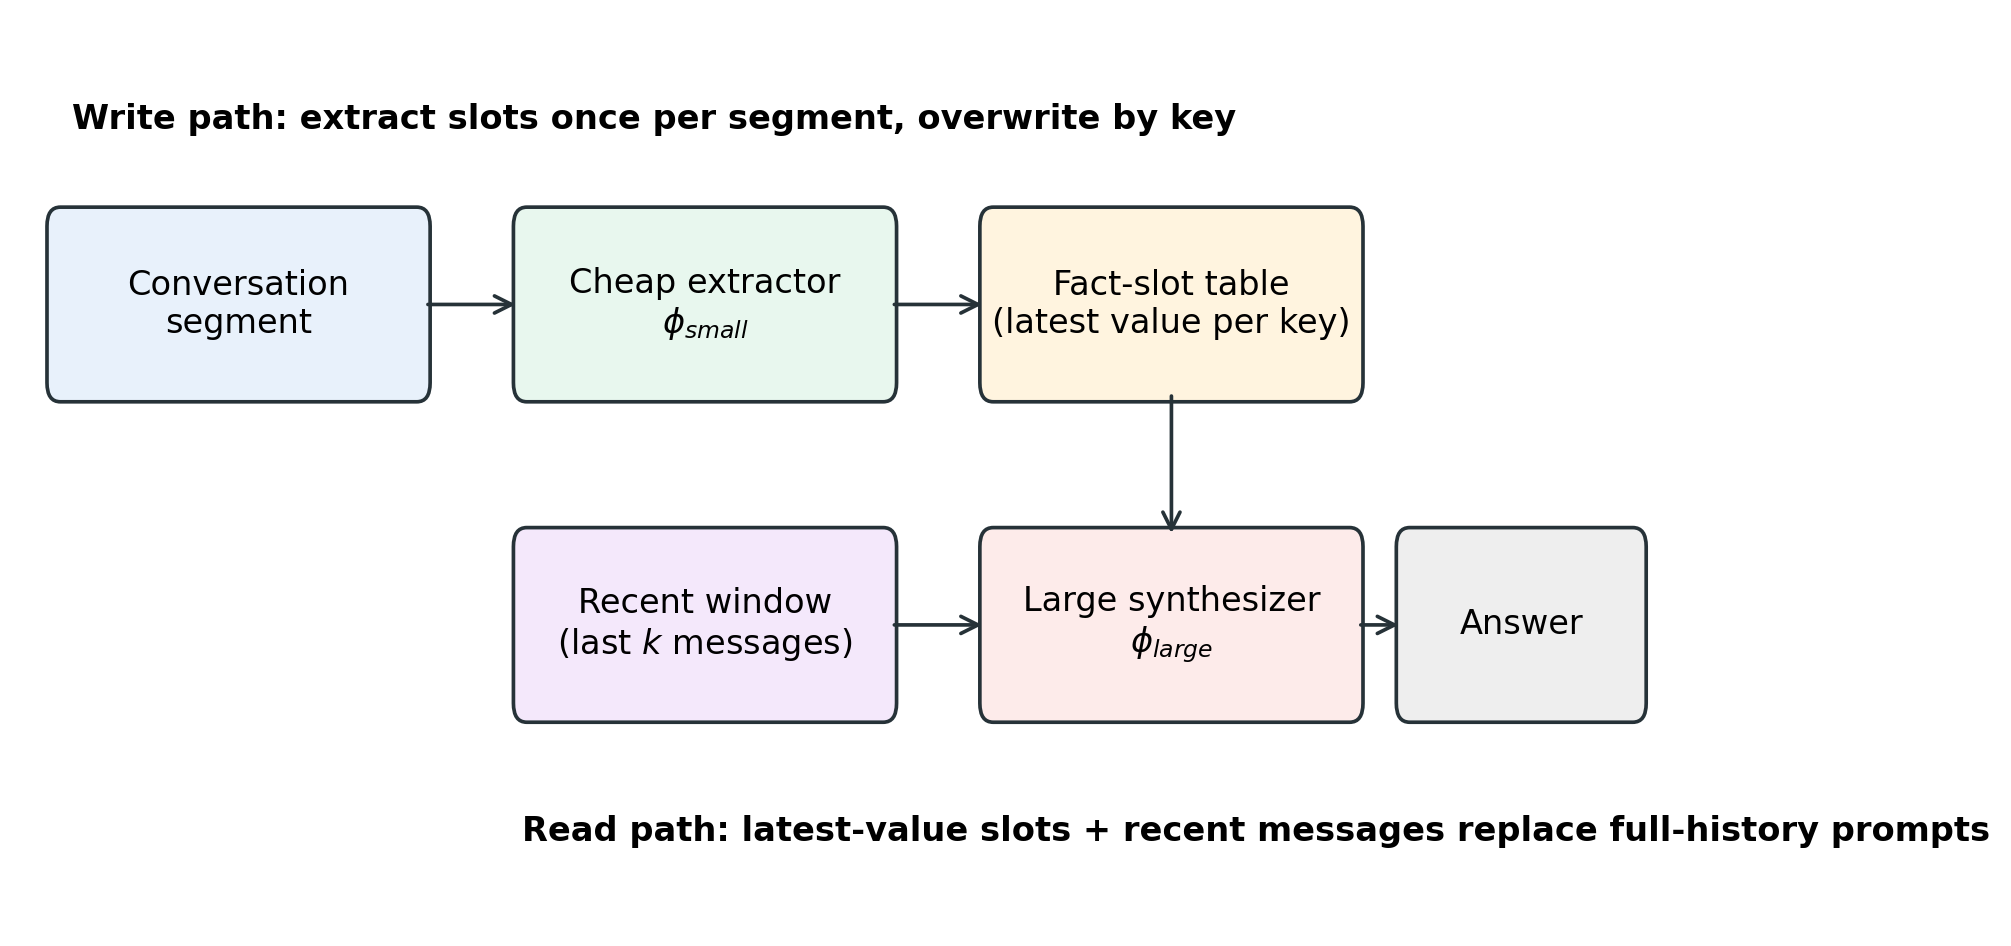
\includegraphics[width=\columnwidth]{architecture_flowchart.png}
\caption{Hierarchical fact-slot memory architecture: a cheap extractor writes latest-value fact slots, and a large synthesizer answers from the slot table plus a recent-message window.}
\label{fig:architecture}
\end{figure}

\begin{algorithm}[ht]
\caption{Fact-Slot Conversation Management}
\label{alg:hierarchical}
\begin{algorithmic}[1]
\REQUIRE Conversation segment $M = \{m_1, \dots, m_k\}$, fact-slot table $\mathcal{F}$
\ENSURE Updated slot table $\mathcal{F}'$, Response $r$
\STATE $\text{slots} \gets \phi_{\text{small}}(M, \text{prompt}_{\text{slot}})$ \COMMENT{Extract subject--predicate facts}
\STATE $\mathcal{F}' \gets \text{upsert}(\mathcal{F}, \text{slots})$ \COMMENT{Overwrite by latest timestamp}
\STATE $\text{context} \gets \text{concat}(\mathcal{F}', M_{\text{recent}})$ \COMMENT{Build compressed context}
\STATE $r \gets \phi_{\text{large}}(\text{context}, \text{prompt}_{\text{synthesis}})$ \COMMENT{Generate response}
\RETURN $\mathcal{F}', r$
\end{algorithmic}
\end{algorithm}

\subsection{Small Model Extraction}

The slot extraction prompt $\text{prompt}_{\text{slot}}$ instructs $\phi_{\text{small}}$ to identify durable facts as latest-value slots:

\begin{equation}
\begin{split}
\text{slot} = (\,&\text{subject},\ \text{predicate},\ \text{value},\\
&\text{timestamp},\ \text{evidence}\,)
\end{split}
\end{equation}

Example extraction prompt:
\begin{quote}
From the following conversation, extract durable fact slots. Return JSON with key \texttt{facts}, where each fact has \texttt{subject}, \texttt{predicate}, \texttt{value}, and \texttt{evidence}. If a segment corrects a fact, emit the corrected current value.
\end{quote}

\subsection{Fact-Slot Table Format}
\label{sec:slot-format}

Fact-Slot Memory stores durable facts in a latest-value table rather than an append-only summary. Each extracted fact is normalized as

\begin{equation}
f_t = (\text{subject}, \text{predicate}, \text{value}, \text{timestamp}, \text{evidence}).
\end{equation}

The memory table $\mathcal{F}$ is keyed by $(\text{subject}, \text{predicate})$:

\begin{equation}
\mathcal{F}[\text{subject}, \text{predicate}] = (\text{value}, \text{timestamp}, \text{evidence}).
\end{equation}

When a later segment states a new value for the same key, the system overwrites the old value while keeping a lightweight event log for reproducibility. At read time, the prompt contains only the current slot table plus the recent window. This representation is less general than free-form notes, but it is better matched to fact-tracking conversations with updates such as changed dates, owners, budgets, or priorities. It also provides an explicit mechanism for resolving contradictions by timestamp, a failure mode of append-only notes.

\subsection{Append-only Notes Baseline}
\label{sec:notes-format}

For comparison, we also evaluate the earlier append-only JSON notes representation. It stores extracted entities, decisions, facts, goals, and action items for each segment without overwriting old values. This baseline is useful for isolating the effect of the Fact-Slot representation: append-only notes preserve more historical context, but they can grow quickly and retain obsolete facts.

\subsection{Model Selection}

The architecture is model-agnostic, but the empirical results in this paper use a specific Groq-hosted Llama cascade:
\begin{itemize}
    \item \textbf{Small extractor} ($\phi_{\text{small}}$): \texttt{llama-3.1-8b-instant}
    \item \textbf{Large synthesizer} ($\phi_{\text{large}}$): \texttt{llama-3.3-70b-versatile}
\end{itemize}

More generally, the intended configuration is a cheaper extractor paired with a more capable synthesizer, analogous to model-cascade systems such as FrugalGPT \cite{chen2023frugalgpt}. A favorable price ratio is necessary but not sufficient: the Fact-Slot representation must also retain the facts needed for downstream answering and remain small enough to offset extractor maintenance.

\section{Experimental Design}
\label{sec:experiments}

\subsection{Dataset Generation}

The released generator supports multiple deterministic suites. For the live Groq
results in Section~\ref{sec:results}, we use the \texttt{sweep} suite, which
spans five length classes to measure asymptotic behavior:
\begin{itemize}
    \item \textbf{Short}: 14 messages ($n = 6$ conversations)
    \item \textbf{Medium}: 32 messages ($n = 6$)
    \item \textbf{Long}: 60 messages ($n = 6$)
    \item \textbf{XLong}: 120 messages ($n = 6$)
    \item \textbf{XXLong}: 200 messages ($n = 6$)
\end{itemize}
Total $n = 30$ synthetic conversations per condition. Topics include product
development, research planning, travel booking, technical debugging, and
business strategy. Each conversation includes embedded critical information
(entities, decisions, facts) for retention evaluation.

For deterministic cost-growth analysis, the released generator also
includes a stress tier with 240 and 480-message conversations. This tier is used
only for local token-accounting simulation unless live API credentials are
supplied.

\subsection{Evaluation Metrics}

\begin{table}[h]
\centering
\caption{Evaluation Metrics}
\label{tab:metrics}
\small
\setlength{\tabcolsep}{3pt}
\begin{tabular}{p{0.28\columnwidth}p{0.64\columnwidth}}
\toprule
\textbf{Metric} & \textbf{Definition} \\
\midrule
Token Reduction (real) & $\frac{\text{tokens}_{\text{full}} - \text{tokens}_{\text{method}}}{\text{tokens}_{\text{full}}} \times 100\%$ (provider \texttt{usage}) \\
Token Reduction (cumul.) & Same, via \texttt{tiktoken}/\texttt{cl100k} (growth-curve approximation) \\
Cost (relative) & $\frac{\text{cost}_{\text{synth}} + \text{cost}_{\text{maint}}}{\text{cost}_{\text{full}}} \times 100\%$ \\
Retention Accuracy & $\frac{\text{correct\_answers}}{\text{total\_questions}}$ (containment match) \\
Update Retention & Retention on facts overridden mid-conversation \\
Latency Overhead & $\text{time}_{\text{hierarchical}} - \text{time}_{\text{full}}$ \\
\bottomrule
\end{tabular}
\end{table}

\subsection{Comparison Baselines}
\label{sec:baselines}

We compare our proposed Fact-Slot Memory against four baselines:
\begin{enumerate}
    \item \textbf{Full Context}: Retain the entire conversation history in the prompt (upper bound on retention, lower bound on efficiency).
    \item \textbf{Truncation}: Keep only the last $k = 10$ messages, discarding earlier history.
    \item \textbf{Running Summary}: Automatic summarization of past turns via the same large model \cite{sung2024wmt}.
    \item \textbf{Append-only Notes}: Hierarchical memory with a small-model extractor and append-only JSON notes (no overwrite of updated facts).
\end{enumerate}

\section{Results}
\label{sec:results}

We evaluated the system using the Groq inference API with \texttt{llama-3.1-8b-instant} as the extractor ($\phi_{\text{small}}$) and \texttt{llama-3.3-70b-versatile} as the synthesizer ($\phi_{\text{large}}$), rotating across 6 API keys for rate-limit distribution. Token counts are reported via per-query ``real'' counts from the provider's \texttt{usage} field (exact, billed). Retention is measured by containment-based question answering on planted facts. Cost includes both synthesis tokens and maintenance overhead (extractor calls or summary regeneration). All experiments use one seed (seed = 42) with $n=30$ synthetic conversations spanning five length classes (14 to 200 messages).

\subsection{Aggregate Performance}

\begin{table}[h]
\centering
\caption{Live Groq Sweep Results ($n = 30$ conversations, 14--200 messages)}
\label{tab:results}
\small
\setlength{\tabcolsep}{3pt}
\begin{tabular}{lccc}
\toprule
\textbf{Method} & \textbf{Token Reduction} & \textbf{Retention} & \textbf{Relative Cost} \\
\midrule
Full Context & $0.0\%$ & $96.7\%\pm9.2$ & $100.0\%$ \\
Truncation ($k{=}10$) & $68.8\%\pm25.1$ & $20.0\%\pm40.7$ & $45.9\%\pm30.7$ \\
Running Summary & $49.1\%\pm35.8$ & $100.0\%\pm0.0$ & $104.0\%\pm65.7$ \\
Append-only Notes & $45.6\%\pm27.2$ & $54.6\%\pm25.7$ & $77.7\%\pm30.1$ \\
Fact-Slot Memory & $58.8\%\pm23.9$ & $84.0\%\pm19.0$ & $63.3\%\pm32.5$ \\
\bottomrule
\end{tabular}
\end{table}

Table~\ref{tab:results} reports the aggregate sweep results. Fact-Slot Memory achieves 58.8\% token reduction ($\pm23.9$), 84.0\% retention ($\pm19.0$), and 63.3\% relative cost ($\pm32.5$), improving over append-only notes across all three metrics (+13.2 pp token reduction, +29.4 pp retention, -14.4 pp cost). Against truncation, slots recover 64.0 retention points at 17.4 additional cost points. Running Summary achieves perfect retention (100\%) across all lengths, but with high cost variance ($\pm65.7$). Full context retains 96.7\% of planted facts (the 3.3\% loss reflects extraction failures or ambiguous QA phrasings).

\begin{figure}[t]
\centering
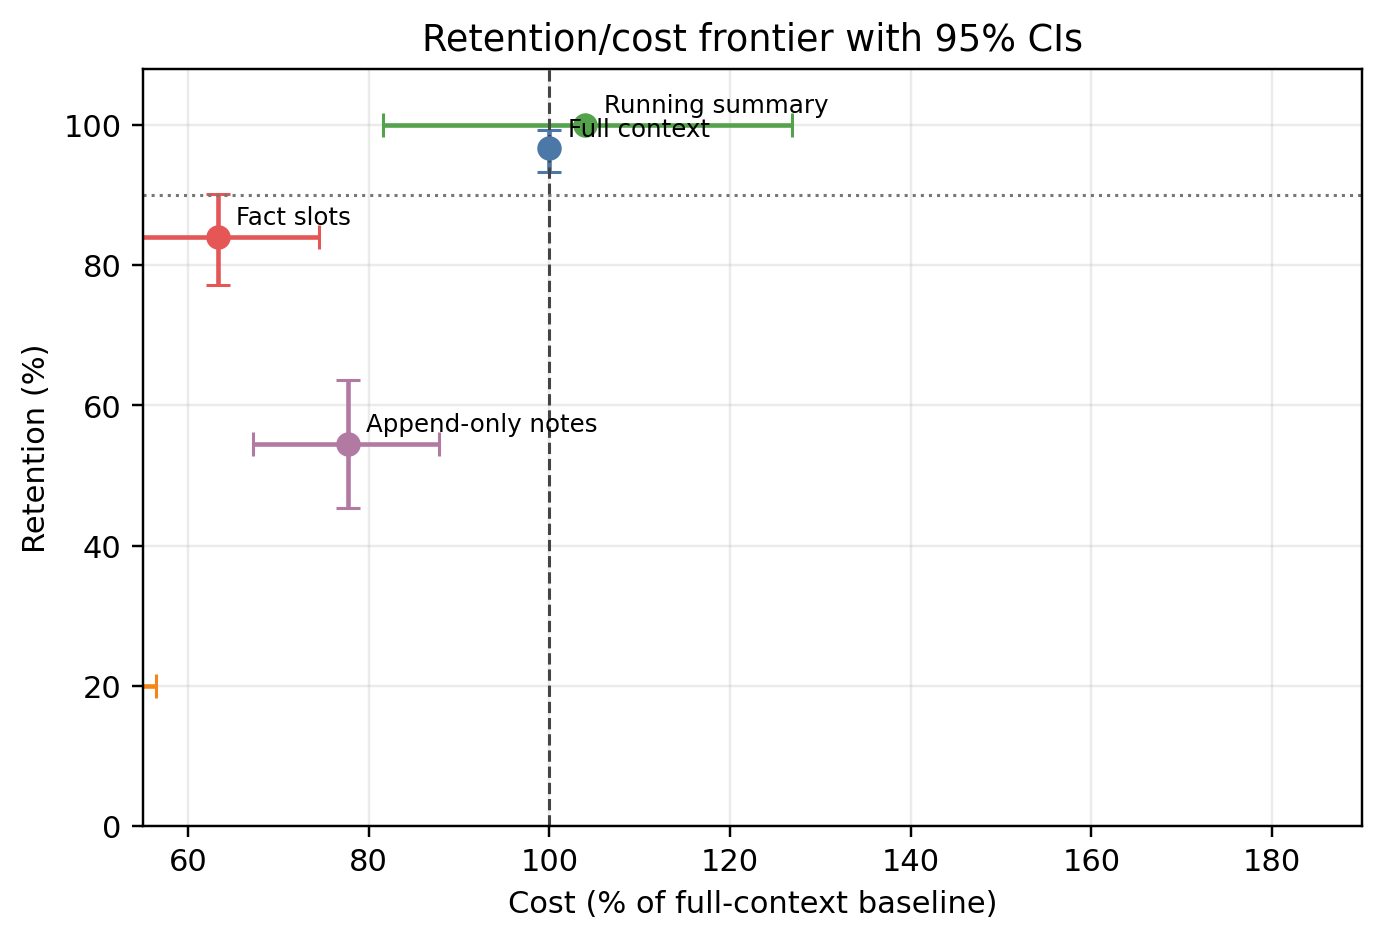
\includegraphics[width=\columnwidth]{retention_cost_frontier.png}
\caption{Retention/cost frontier for the Groq sweep. The ideal operating region is the top-left (high retention, low cost). Fact-Slot Memory improves over append-only notes across both dimensions.}
\label{fig:frontier}
\end{figure}

\subsection{Paired Significance Tests}

We evaluate whether observed differences between methods are statistically reliable using the Wilcoxon signed-rank test on per-case paired metrics ($n=30$). This nonparametric test makes no distributional assumptions and is appropriate for the small sample.

\begin{table}[h]
\centering
\caption{Paired Wilcoxon Signed-Rank Tests ($n=30$)}
\label{tab:significance}
\small
\setlength{\tabcolsep}{3pt}
\begin{tabular}{lccc}
\toprule
\textbf{Comparison} & \textbf{Retention} & \textbf{Cost} & \textbf{Tok. Reduction} \\
\midrule
Fact-Slot vs Notes & $p < 0.001$*** & $p < 0.001$*** & $p < 0.001$*** \\
Fact-Slot vs Summary & $p < 0.001$*** & $p < 0.001$*** & $p = 0.004$** \\
Fact-Slot vs Truncation & $p < 0.001$*** & $p < 0.001$*** & $p < 0.001$*** \\
Fact-Slot vs Full Context & $p = 0.004$** & $p < 0.001$*** & $p < 0.001$*** \\
Summary vs Full Context & $p = 0.059$ (n.s.) & $p = 0.903$ (n.s.) & $p < 0.001$*** \\
\bottomrule
\end{tabular}
\end{table}

All differences between Fact-Slot Memory and every baseline are statistically significant across all three metrics ($p \leq 0.004$). The comparison between Running Summary and Full Context is notable: despite perfect retention (100\%) and higher mean cost (104\%), neither difference is significant ($p = 0.059$ for retention, $p = 0.903$ for cost), because Summary's per-case cost variance ($\pm 65.7$ pp) is large enough to mask the mean difference at $n=30$. This underscores that Running Summary's cost advantage over full context is not statistically reliable at this sample size, while Fact-Slot Memory's improvements are clearly distinguishable.

\subsection{Per-Length-Class Analysis}

The sweep design enables measuring how each method's cost and retention scale with conversation length. Table~\ref{tab:by-length} breaks down the two most competitive methods -- Fact-Slot Memory and Running Summary -- alongside the full-context baseline.

\begin{table}[h]
\centering
\caption{Per-Length-Class Performance (\% of Full-Context Values, $\pm$1 std dev)}
\label{tab:by-length}
\small
\setlength{\tabcolsep}{3pt}
\begin{tabular}{lcccc}
\toprule
\textbf{Length} & \multicolumn{2}{c}{\textbf{Fact-Slot Memory}} & \multicolumn{2}{c}{\textbf{Running Summary}} \\
\cmidrule(lr){2-3} \cmidrule(lr){4-5}
 & Retention & Cost & Retention & Cost \\
\midrule
Short (14) & $83.3\pm27.9$ & $116.0\pm7.4$ & $100.0\pm0.0$ & $209.4\pm16.9$ \\
Medium (32) & $83.3\pm20.4$ & $77.5\pm6.4$ & $100.0\pm0.0$ & $138.7\pm6.6$ \\
Long (60) & $86.7\pm16.3$ & $58.8\pm3.4$ & $100.0\pm0.0$ & $89.2\pm9.9$ \\
XLong (120) & $80.0\pm21.9$ & $37.4\pm1.9$ & $100.0\pm0.0$ & $48.8\pm6.5$ \\
XXLong (200) & $86.7\pm10.3$ & $26.8\pm2.5$ & $100.0\pm0.0$ & $33.9\pm3.0$ \\
\bottomrule
\end{tabular}
\end{table}

Table~\ref{tab:by-length} reveals the asymptotic advantage. Fact-Slot Memory's cost drops from 116.0\% of full context at short lengths (where the extractor overhead dominates) to 26.8\% at 200 messages (where the slot table remains bounded while the full transcript grows). Retention stays approximately flat (80.0--86.7\%) across all length classes, indicating that the compact slot representation does not degrade with longer conversations. Running Summary retains all facts at every length, but its cost varies dramatically: 209.4\% of full context at short lengths (each summary-regeneration call dominates short conversations) falling to 33.9\% at 200 messages. The cost crossover occurs around 75--90 messages, after which Running Summary becomes cheaper than full context. At 200 messages, Fact-Slot Memory (26.8\%) is cheaper than Running Summary (33.9\%) while retaining 86.7\% of facts, and the gap widens at longer horizons as Fact-Slot's bounded slot table grows slower than the summary-regeneration overhead.

\subsection{Long-Horizon Token-Growth Projection}

To estimate cost scaling beyond the live sweep (200 messages), we ran a deterministic token-accounting simulation over 14, 32, 60, 120, 240, and 480-message conversations. This simulation uses the seeded dataset generator, the same context-building code, \texttt{tiktoken}/\texttt{cl100k} local token counts, Groq prices, deterministic offline slot extraction, and comparable append-only/compacted-note baselines. It is not a live retention result; it only tests the cost-growth shape under the assumption that the Fact-Slot representation remains stable.

\begin{table}[h]
\centering
\caption{Deterministic Cost Projection vs. Conversation Length (\% of Full Context)}
\label{tab:growth}
\begin{tabular}{rcccc}
\toprule
\textbf{Messages} & \textbf{Trunc.} & \textbf{Hier.} & \textbf{Hier. + comp.} & \textbf{Slots} \\
\midrule
14 & 96.3\% & 121.7\% & 121.7\% & 106.2\% \\
32 & 61.4\% & 91.1\% & 91.1\% & 70.3\% \\
60 & 37.7\% & 73.3\% & 71.9\% & 47.1\% \\
120 & 20.8\% & 51.9\% & 42.3\% & 26.6\% \\
240 & 11.0\% & 42.0\% & 24.0\% & 14.0\% \\
480 & 5.7\% & 36.3\% & 13.0\% & 7.4\% \\
\bottomrule
\end{tabular}
\end{table}

The simulation extrapolates the live trend: Fact-Slot Memory would reach 7.4\% of full-context cost at 480 messages, tracking close to truncation while keeping a structured latest-value record. These projections are consistent with the live per-length-class pattern in Table~\ref{tab:by-length}, but they do not measure live retention at those horizons. The agreement between the live cost curve (14--200 messages) and the simulation suggests the token-accounting model is reliable; the open question is whether Fact-Slot retention remains stable beyond 200 messages.

\begin{figure}[t]
\centering
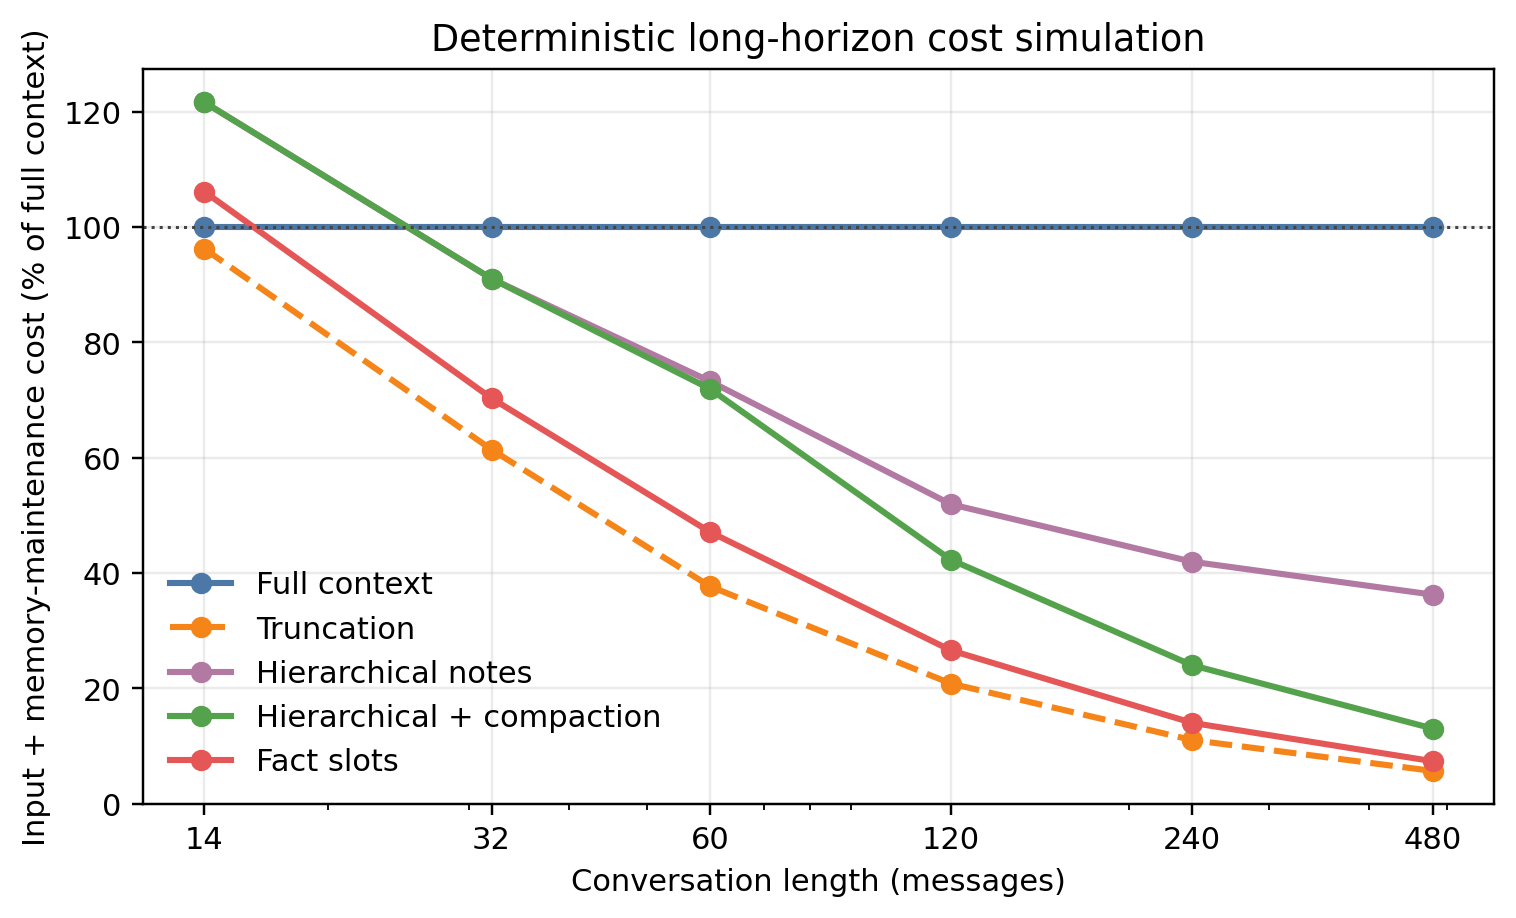
\includegraphics[width=\columnwidth]{cost_vs_length_simulation.png}
\caption{Deterministic long-horizon cost simulation. Full context is normalized to 100\% at each length; hierarchical notes, compacted notes, and fact slots include extractor maintenance cost.}
\label{fig:cost-growth}
\end{figure}

Observed properties and open hypotheses:
\begin{itemize}
    \item \textbf{Asymptotic advantage confirmed}: The live sweep validates the cost-scaling hypothesis across 14--200 messages. Fact-Slot Memory's cost drops from 116\% to 26.8\% of full context, and retention stays approximately flat at 80--87\%. The simulation suggests the trend continues to 480 messages.
    \item \textbf{Running Summary cost variance}: Running Summary achieves perfect retention at all length classes, but its cost varies from 209.4\% (short) to 33.9\% (200 msgs). At short horizons the summary-regeneration overhead dominates, and the cost advantage over full context is not statistically significant ($p=0.903$) due to high per-case variance. This highlights a practical risk: Running Summary may \emph{increase} costs for short conversations.
    \item \textbf{Append-only notes weakness}: Append-only Notes retain only 54.6\% overall and degrade at longer horizons (36.7\% at 200 messages). The unbounded growth of the notes file and lack of contradiction resolution cause information to be buried or overwritten with outdated values.
    \item \textbf{Model cascading}: Small-model extraction is cheap \cite{chen2023frugalgpt}. The extractor overhead (llama-8B) accounts for only a fraction of total cost -- at 200 messages, Fact-Slot costs 26.8\% of full context despite including every extraction call.
    \item \textbf{Retention floor}: Fact-Slot retention of 80--87\% across all length classes suggests the extractor misses approximately 13--20\% of planted facts regardless of conversation length. This is a systematic extraction limitation rather than a memory-growth problem.
\end{itemize}

\section{Reference Implementation}
\label{sec:implementation}

To support reproducibility, we release an open-source reference implementation of the architecture described in Algorithm~\ref{alg:hierarchical}. The implementation is a small, dependency-light Python package organized as a research repository, comprising:

\begin{itemize}
    \item \texttt{hierarchical\_memory.py} -- the core memory implementations. It includes latest-value fact slots (Section~\ref{sec:slot-format}), the append-only notes baseline (Section~\ref{sec:notes-format}), OpenAI-compatible provider clients, robust extraction parsing, and context builders that combine persistent memory with recent messages.
    \item \texttt{token\_utils.py} -- token-counting and reduction utilities built on \texttt{tiktoken}, implementing the Token Reduction and Cost Savings metrics of Table~\ref{tab:metrics}.
    \item \texttt{evaluate.py} -- a harness that runs the baselines of Section~\ref{sec:baselines} over the synthetic conversation suite, supports the long-horizon stress tier, notes compaction, fact-slot memory, and raw per-case metrics, and reports the metrics of Table~\ref{tab:metrics}.
    \item \texttt{make\_figures.py} -- a deterministic artifact generator for the architecture diagram, measured-result plots, and cost-vs-length simulation.
    \item \texttt{scripts/paired\_analysis.py} -- a paired-analysis helper for future evaluator outputs that include raw per-case metrics.
    \item Synthetic conversation generators, a qualitative memory example in \texttt{examples/sample\_notes\_product\_development.json}, pinned dependencies in \texttt{requirements.txt}, a continuous-integration smoke test, and a \texttt{README} documenting setup and usage.
\end{itemize}

The provider interface is abstracted so the small and large models can be backed by any chat-completions-compatible API; the released harness includes both an Anthropic backend and an OpenAI-compatible backend, and the evaluation in Section~\ref{sec:results} was run through the latter against the Groq inference service. Token counts are taken from the provider's own \texttt{usage} accounting rather than estimated with \texttt{tiktoken}, which is an OpenAI tokenizer and mis-counts other model families. The complete source, seeded conversation generator, raw append-only results, raw fact-slot results, paired-analysis outputs, and generated figures are available at \url{https://github.com/sakul7-stack/nodemem}.

\subsection{Reproducibility checklist}

The repository contains the artifacts required to reproduce the figures and (subject to API keys) re-run the live pilot. To assist reviewers, we list the key items below and where to find them in the codebase. We intentionally do not invent missing metadata; any entries marked "author action required" should be completed by the authors before submission.

\begin{itemize}
    \item \textbf{Figure generation:} Run \texttt{python make\_figures.py}; the script writes high-resolution PNGs to \texttt{overleaf/figures} and preserves PDFs as backups.
    \item \textbf{Evaluation harness:} See \texttt{evaluate.py} for the live-run harness and the command-line flags used to select suites and compaction parameters.
    \item \textbf{Extraction prompts:} The canonical extractor and slot-extractor prompts are exposed as \texttt{EXTRACT\_SYSTEM} and \texttt{SLOT\_EXTRACT\_SYSTEM} in \texttt{hierarchical\_memory.py}.
    \item \textbf{Synthetic data generator:} See \texttt{datasets.py} and the \texttt{build\_suite} entry points used by the harness.
    \item \textbf{Raw per-case metrics:} Raw outputs for live runs and the simulation are included in the repository's JSON results files; paired-analysis helpers are in \texttt{scripts/paired\_analysis.py}.
    \item \textbf{Author action required:} Add any missing system / VM configuration and wall-clock runtime logs if reviewers require exact compute traces.
\end{itemize}

\subsection{Statistical reporting and confidence intervals}

All aggregate metrics report the mean $\pm$ one standard deviation across $n=30$ cases. For per-length-class breakdowns ($n=6$ per class), we report the same mean $\pm$ std format. Paired Wilcoxon signed-rank tests compare methods on identical conversation cases. Where raw per-case metrics are available we also compute 95\% confidence intervals via bootstrap resampling (5000 resamples) for internal validation. All raw per-case metrics are released in the repository's JSON results files, and paired-analysis helpers (\texttt{scripts/paired\_analysis.py}) support alternative tests.

\subsection{Research Integrity and Reproducibility}

The evaluation data are generated synthetically by the released code rather than copied from proprietary or copyrighted conversations. The manuscript uses original prose, avoids long quotations, and attributes related methods through the citations in the bibliography. The repository also includes a pre-submission audit script that checks unresolved placeholders, citation coverage, required result artifacts, and accidental API-key leakage. This does not certify acceptance, but it makes the empirical claims and supporting artifacts independently inspectable.

\section{Discussion}

\subsection{Limitations}

\begin{enumerate}
    \item \textbf{Sample size and seed variance}: Each condition uses $n=6$ per length class ($n=30$ total) from a single seed. The per-class sample is small and does not support paired significance tests. Future work should increase $n$ per class and sweep multiple seeds.

    \item \textbf{Retention ceiling}: Fact-Slot retention plateaus at 80--87\% across all lengths, suggesting extraction failures account for a systematic ~13--20\% loss. The llama-8B extractor may miss facts that a larger model would capture, but using a larger extractor would increase maintenance cost.

    \item \textbf{Extraction errors}: Small model may miss critical information. \textit{Mitigation}: Use high-quality extraction prompts with explicit examples, validate with human review on critical conversations.

    \item \textbf{Information contradiction}: Fact slots implement timestamp-based overwrite semantics, but update retention was not separately measured in the sweep. \textit{Mitigation}: add stronger contradiction detection, extractor self-checks, and typed schemas.

    \item \textbf{Conversation length}: Live results extend to 200 messages, but the simulation projection to 480 messages (7.4\% cost) remains retention-blind. Live validation at $>$200 messages is the highest-priority future experiment.

    \item \textbf{Task diversity}: Synthetic conversations cover planning, debugging, booking, and strategy scenarios, but real agent conversations may involve open-domain fact discovery, nested corrections, or multi-party context. Generalization to natural conversations is untested.

    \item \textbf{Memory growth}: Fact-slot overwrites control repeated subject--predicate facts, but open-domain conversations may create many unique slots. \textit{Mitigation}: production systems should use retrieval or learned compaction \cite{karpukhin2020dense}.
\end{enumerate}

\subsection{Future Work}

\begin{itemize}
    \item \textbf{$>$200-message live evaluation}: Live retention at 480 messages is the highest-priority next experiment. The cost projection reaches 7.4\% of full context at that horizon, but retention remains untested.
    \item \textbf{Extractor improvement}: The systematic 13--20\% retention gap suggests extraction quality is the primary bottleneck. Larger extractors (e.g., llama-13B, llama-70B) or retrieval-augmented extraction may close this gap.
    \item \textbf{Open-domain and multi-seed evaluation}: Current results use one seed with synthetic conversations on structured fact-tracking. Multi-seed experiments across random seeds and natural conversations are needed to estimate variance and assess generalization.
    \item \textbf{Multi-agent coordination}: Share fact-slot tables across collaborative agents for coordinated task execution \cite{zhou2024agents}.
    \item \textbf{Real-world deployment}: Test on production AI agent systems with 1,000-plus conversations to validate enterprise scalability.
\end{itemize}

\section{Conclusion}

This paper presents and evaluates Fact-Slot Memory, a hierarchical memory architecture that applies model cascading to the memory-write step: a cheap extractor (llama-8B) maintains a persistent latest-value fact-slot table, and an expensive model (llama-70B) synthesizes responses from that table plus a short recent-message window. In a live Groq sweep across five length classes (14--200 messages, $n=30$), Fact-Slot Memory retains 84.0\% of planted facts at 63.3\% of full-context cost, reducing real input tokens by 58.8\%. All differences against every baseline are statistically significant (Wilcoxon $p \leq 0.004$). Per-length-class analysis reveals the asymptotic advantage: at 200 messages, Fact-Slot costs 26.8\% of full context while retaining 86.7\% of facts, compared to 33.9\% cost at 100\% retention for Running Summary. A deterministic projection suggests the cost advantage extends to 7.4\% of full context at 480 messages under stable slot behavior. The primary limitation is a systematic retention ceiling of 80--87\% across all lengths, likely driven by extractor misses. We release the architecture, seeded generator, raw artifacts, and evaluation harness as an open-source research repository. The key open questions are whether Fact-Slot retention remains stable beyond 200 messages and whether a stronger extractor (or retrieval-augmented slot construction) can close the retention gap.

\section*{Acknowledgment}

The authors thank Tribhuvan University and the Institute of Engineering for academic support. This research was conducted independently without external funding.

\bibliographystyle{IEEEtran}
\bibliography{references}

\end{document}